\documentclass[12pt]{article}
\usepackage{amsmath,amssymb}
\usepackage{hyperref}
\usepackage{cite}
\usepackage{graphicx}
\usepackage{hyperref}
\title{Neuron's eye view: inferring features of complex stimuli from neural responses}
\author{Xin (Cindy) Chen, Jeffrey M. Beck & John M. Pearson}
\date{}
\begin{document}
\maketitle

\begin{abstract}
    Experiments that study neural encoding of stimuli at the level of individual neurons typically choose a small set of features present in the world --- contrast and luminance for vision, pitch and intensity for sound --- and assemble a stimulus set that systematically varies along these dimensions. Subsequent analysis of neural responses to these stimuli typically focuses on regression models, with experimenter-controlled features as predictors and spike counts or firing rates as responses. Unfortunately, this approach requires knowledge in advance about the relevant features coded by a given population of neurons. For domains as complex as social interaction or natural movement, however, the relevant feature space is poorly understood, and an arbitrary \emph{a priori} choice of features may give rise to confirmation bias. Here, we present a Bayesian model for exploratory data analysis that is capable of automatically identifying the features present in unstructured stimuli based solely on neuronal responses. Our approach is unique within the class of latent state space models of neural activity in that it assumes that firing rates of neurons are sensitive to multiple discrete time-varying features tied to the \emph{stimulus}, each of which has Markov (or semi-Markov) dynamics. That is, we are modeling neural activity as driven by multiple simultaneous stimulus features rather than intrinsic neural dynamics.  We derive a fast variational Bayesian inference algorithm and show that it correctly recovers hidden features in synthetic data, as well as known encoding results in a pair of well-known neuroscience data sets, including in versus out of response field, faces-selectivity, and direct versus indirect gaze.
\end{abstract}

\section*{Additional Detail}

All code and analysis for the project is available at: \\ \url{https://github.com/pearsonlab/spiketopics}.

\vspace{5mm}

\noindent Inferred features and firing rates for anterior fundus responses to image categories (McMahon et al., 2014, PNAS): \\

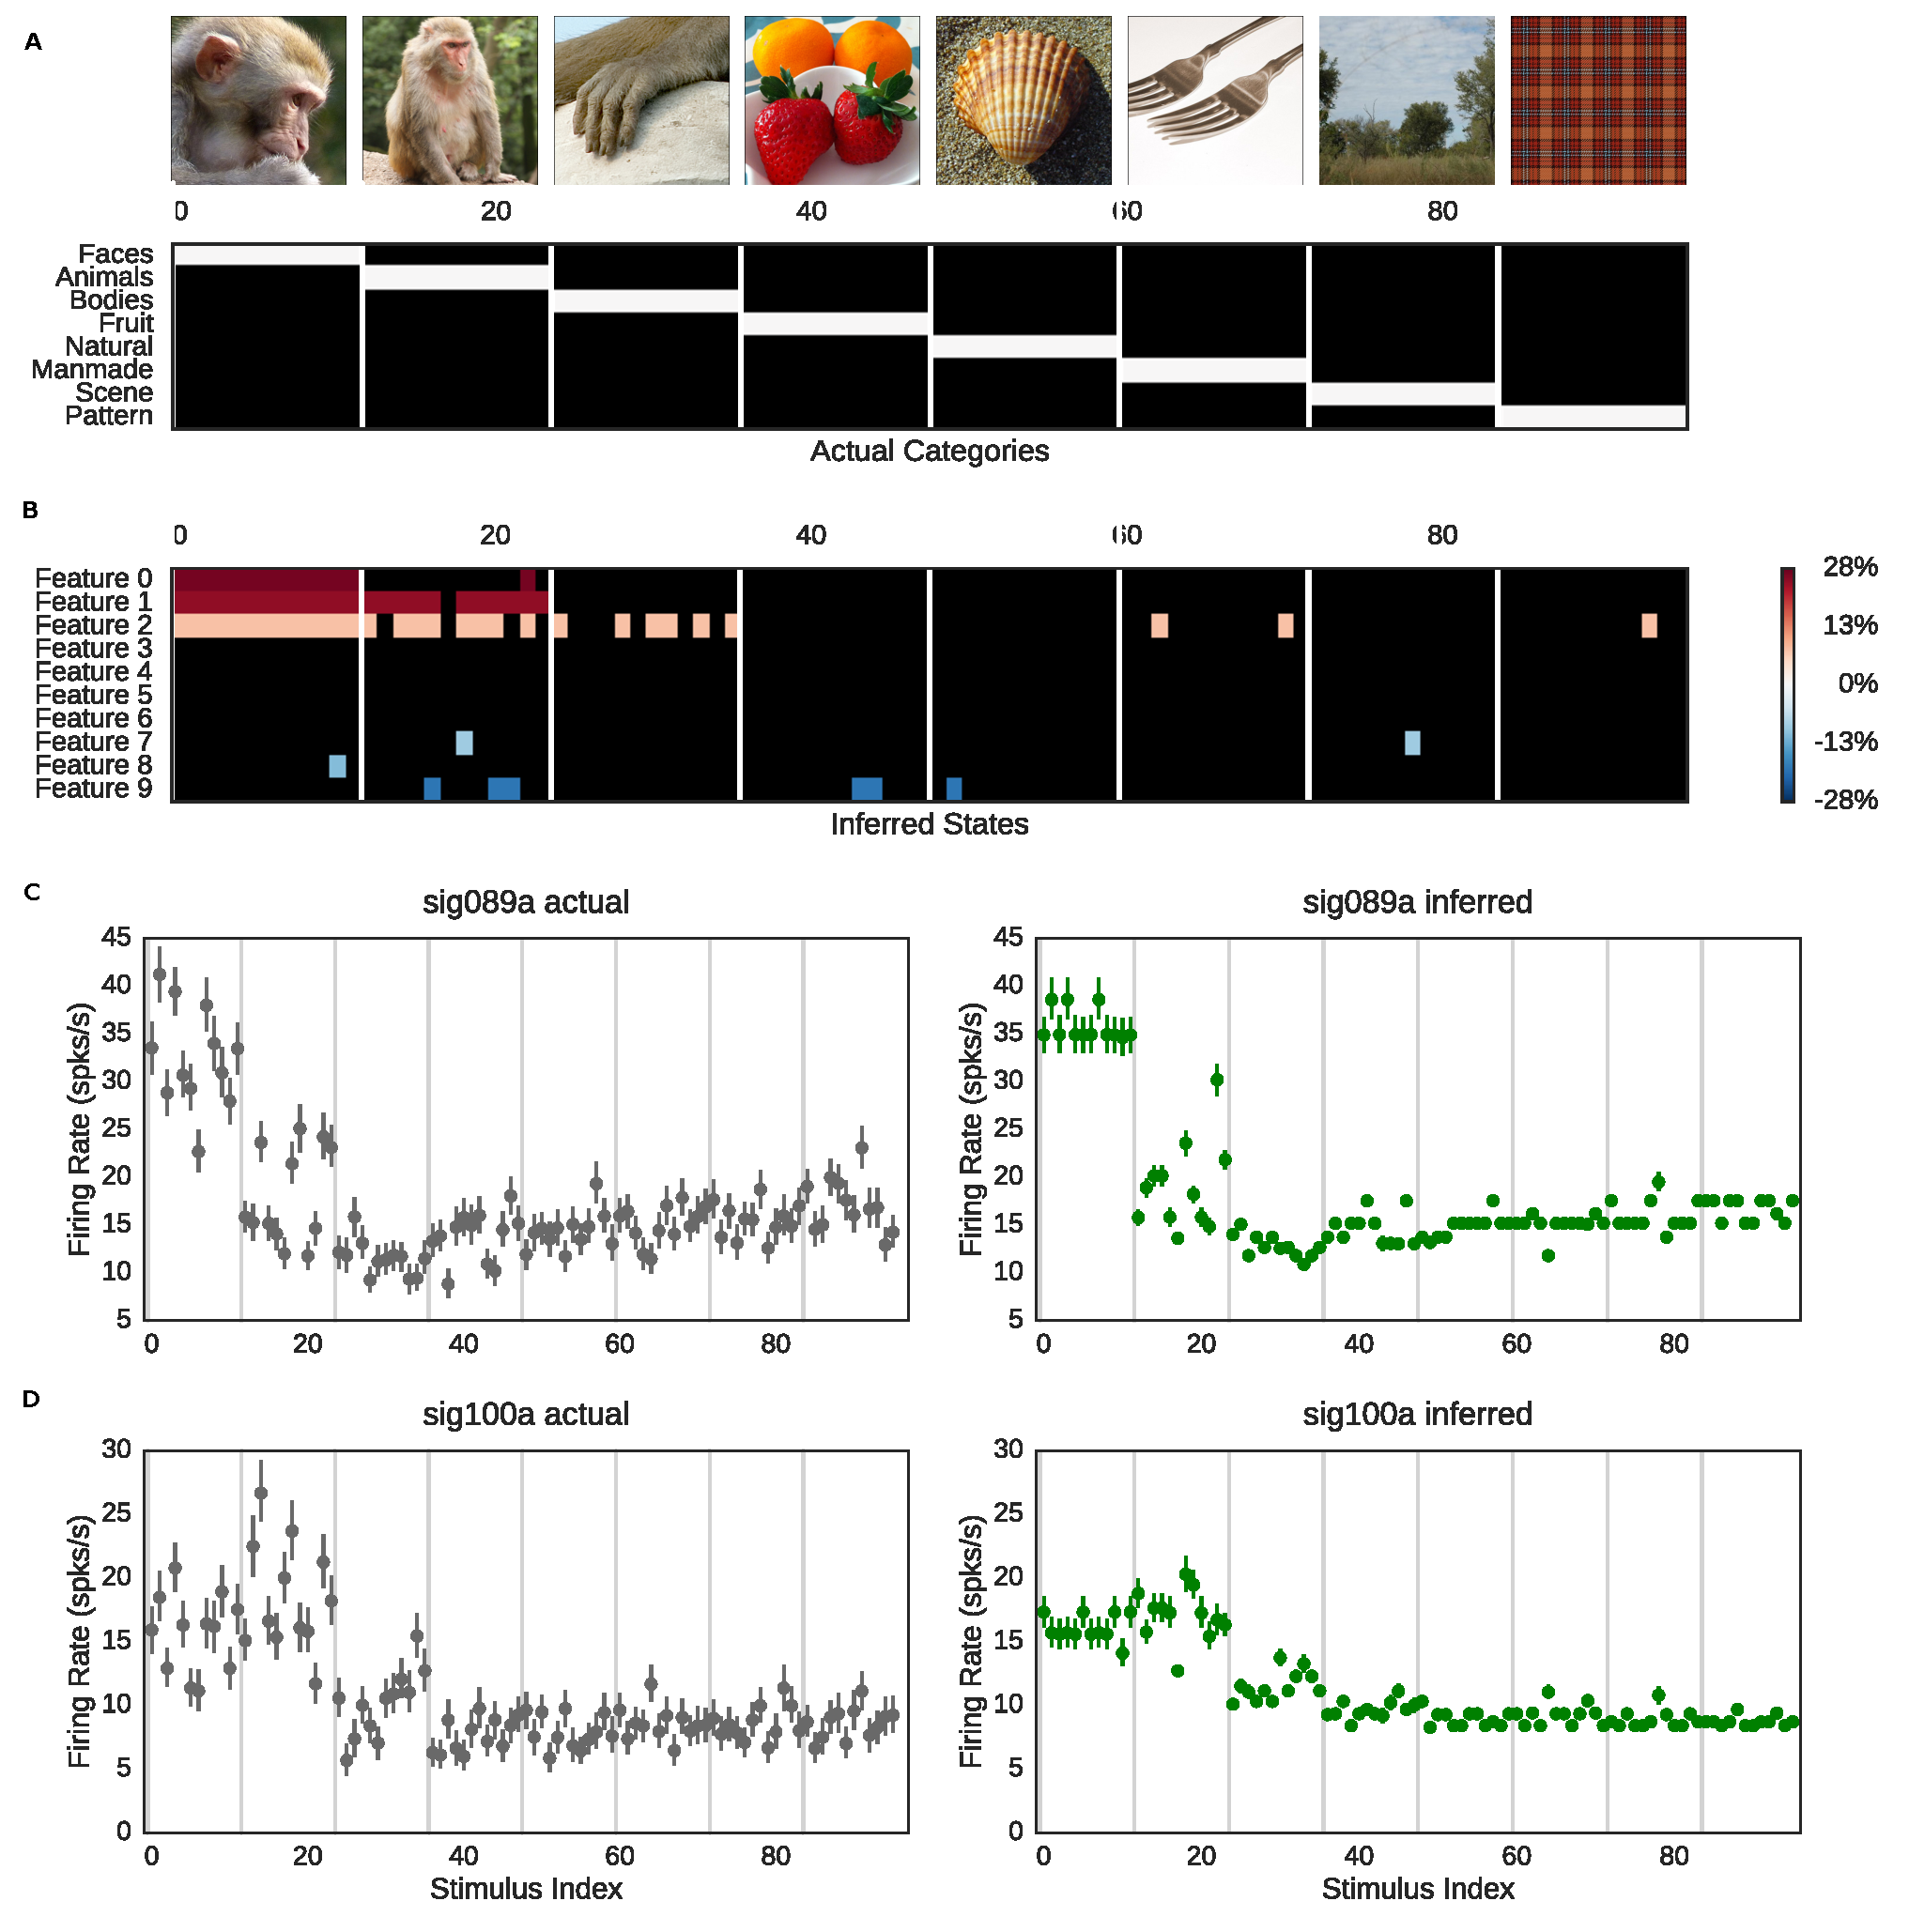
\includegraphics[width=\linewidth]{../plos2016/figures/imgclust}

\end{document}
